\documentclass{article}
\usepackage[utf8]{inputenc}

\title{CS 267-HW1: Optimized DGEMM}
\author{Brian Park, Michael Luo, Iniyaal Kannan }
\date{February 2022}

\usepackage{minted}
\usepackage{algorithm}
\usepackage{algorithmicx}
\usepackage[table]{xcolor} % <==========================================
\usepackage{algpseudocode}

\usepackage{graphicx}
\usepackage[margin=0.70in]{geometry}
\usepackage{listings}


\begin{document}

\maketitle

\section{Introduction}
The goal of this homework is the implement our own DGEMM function for the Cori KNL node. Specifically, we were tasked to reach the highest GFLOPS in matrix-matrix multiplication, as well as analyzing our optimizations. Below, we will explain our optimizations to achieve 28.14\% peak performance of the KNL nodes, with a general all-purpose algorithm rather than different algorithms for different matrix sizes (theoretical peak for KNL is 44.8 GFLOPS).

In the following sections, we will cover Homework 1 in the following order. First, we will go into detail of how our algorithm exactly works, which is greatly inspired from prior work~\cite{10.1007/s10586-018-2810-y}. Then, we will detail and explain the general techniques we used to achieve our speedups, some of which were hinted in the recitation slides. Lastly, we will cover lessons learned, of what techniques worked for us, and what did not.

\section{Our Algorithm}
As we were stuck with the optimizations we figured out from scratch, we searched for relevant research papers to learn techniques from. We found a paper from Lim ~\cite{10.1007/s10586-018-2810-y} to be convenient in helping us exploit all the architecture that the KNL node provides. Lim was able to exploit everything about the KNL node for single core DGEMM, such as optimizing over L1 and L2 cache, repacking matrices, and utilizing all 32 AVX-512 registers to achieve near peak performance of Intel MKL (Math Kernel Library), which is state of the art BLAS library tuned specifically for Intel architectures. He goes on to explain how to parallelize with MIMD and OpenMP, but fortunately the approaches between SIMD and MIMD can be separated. Unfortunately, the paper did not have source code, and instead contained pseudo-code, so it was up to us to use the ideas from Lim and implement it correctly. 

We directly write pseudo code for our algorithm in this section. Our algorithm is simple and takes at most 200 lines of code, which is considered relatively terse for optimized DGEMM algorithms.

Our algorithm consists of two portions. The first algorithm, like the starter code, traverses through matrices $A$ and $B$ in a block matrix format and packs the submatrices together. The second algorithm is the microkernel. We make full use of the 32 vector registers than Intel's KNL CPU offers, allowing for extreme parallelism. 

\subsection{Algorithm 1: Looping through Block Matrices}
\label{sec:blockalg}
Algorithm 1 is directly listed below. Our algorithm directly stacks on top on an existing algorithm proposed by Lim~\cite{10.1007/s10586-018-2810-y}. Like cache blocking in the starter code, this algorithm blocks computations optimizing over L1 and L2 cache. Lim provides derivations of parameters he used. For example, he found the microkernel block size (1620, 31) to be the most optimal on KNL. 

$$k_b \times m_b \times 8 \textnormal{ bytes} \leq \frac{\textnormal{ size}(L2)}{2}$$
$$n_r \times k_b \times 8 \textnormal{ bytes} \leq \frac{\textnormal{ size}(L1)}{2}$$

We know that the L1 cache is 32KiB and the L2 cache is 1024KiB. Thus, the parameters of the microkernel size makes sense.

The first loop iterates over steps of $k_b$. This parameter is recommended to be made as large as possible to reduce the overhead induced by updating $\hat{C}$ at the end of the innermost loop. Then it iterates over steps of $m_b$, which is recommended to be so that $\tilde{A}$ takes up less than half of the L2 cache. We'll later see why that is the case in the microkernel. The next two iterations in steps of $n_r$ and $m_r$ are for blocking on the microkernel. $\hat{B}$ is also recommended to fit less than half of the L1 cache, as it is used $\frac{m_b}{m_r}$ times. These blocking parameters are found to be most optimal, as they are also derived from Goto \cite{10.1145/1356052.1356053}.

Our algorithm is different from ~\cite{10.1007/s10586-018-2810-y} in many ways. First, ~\cite{10.1007/s10586-018-2810-y} packs matrices in a resorted order that makes it so that it only needs to repack into $\tilde{A}$ and $\tilde{B}$ once each and then conveniently index off of $\tilde{A}$ and $\tilde{B}$ to retrieve $\hat{A}$ and $\hat{B}$, as they would be resorted into their respective axis ordering, and then reordered in the other axis in blocks. E.g. $\hat{B}$ is in row major order, but then blocks of $\hat{B}$ are sorted in column major in $\tilde{B}$. Originally, we had trouble repacking, as we actually repacked 3 times originally. Once for each $\tilde{A}$ and $\tilde{B}$, and then once again for $\hat{B}$ to convert the matrices from column major to row major. We saw this extra packing routine costly, but then were able to remove it by efficiently packing B to be row-major order. Although this doesn't follow the design of matrices mentioned by Lim, the resorting order was not explicitly mentioned and we improvised with what was given to us in the starter code with column major order matrices. We only assumed Lim was resorting the matrices with mixed axis orderings, as we did not achieve the full performance Lim stated.

\begin{algorithm}[H]
\label{alg:algorithm1}
\caption{Matrix Multiplication Algorithm, modified from ~\cite{10.1007/s10586-018-2810-y}}
\begin{algorithmic}
    \Require Matrix $A$,$B$,$C$ in  column-order
    \Require Matrix Size $lda$
    \Require $k_b$, $m_b$, $m_r$, $n_r$ for splitting Matrix $A$, $B$ 
    \Require $c_b$ for Matrix chunking $\tilde{B}$
    \State $\tilde{A}$ = malloc($k_b \cdot m_b \cdot 8$)
    \State $\tilde{B}[]$ = [malloc($c_b * k_b$),malloc($c_b * k_b$), ...] \Comment{$\tilde{B}[]$ is of length $lda/c_b$}
    \For{$p = 0, ..., k - 1$ \textit{in steps of $k_b$}}
        \State Pack $B(p : p + k_b - 1, 0: n - 1)$ into $\tilde{B}[]$ \Comment{Row-Order}
        \For{$i = 0, ..., m - 1$ \textit{in steps of $m_b$}}
            \State Pack $A(i : i + m_b - 1, p: p + k_b - 1)$ into $\tilde{A}$ \Comment{Column-Order}
            \For{$jr = 0, ..., n - 1$ \textit{in steps of $n_r$}}
                \For{$ir = 0, ..., m_b - 1$ \textit{in steps of $m_r$}}
                    \State $\hat{A} = \tilde{A} + ir;$
                    \State $\hat{B} = \tilde{B}[jr/c_b] + jr\%c_b;$
                    \State $\hat{C} += \hat{A}\times\hat{B};$ \Comment{Algorithm 2: Microkernel}
                    \State Update $C$ using $\hat{C}$;
                \EndFor    
            \EndFor    
        \EndFor    
    \EndFor
\end{algorithmic}
\end{algorithm}

A visual representation of how these matrices are looped over and packed is below:

\begin{figure}
  \centerline{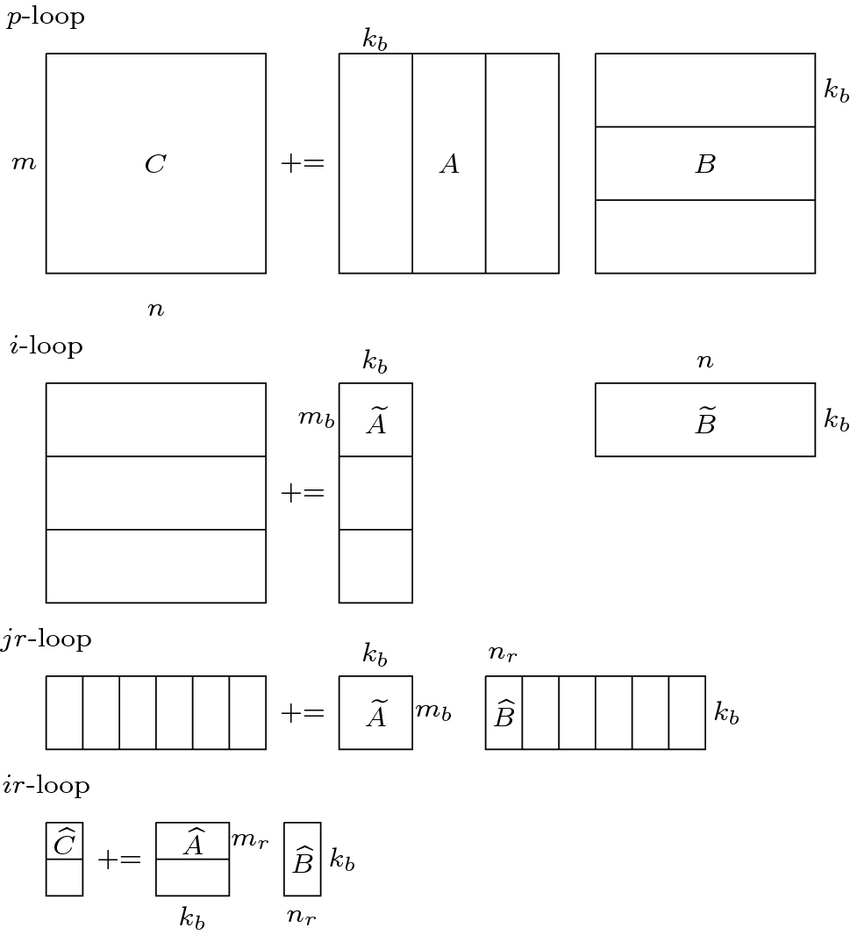
\includegraphics[width=4in]{figures/Illustration-of-Algorithm-1.png}}
  \caption{Illustration of Algorithm 1 ~\cite{10.1007/s10586-018-2810-y}}
\end{figure}

\newpage

\subsection{Algorithm 2: Fast Microkernel}
Algorithm 2 consisted of implementing a micro-kernel that is able to exploit ILP (instruction level parallelism), DLP (data level parallelism), and the memory hierarchy. Interestingly, Lim~\cite{10.1007/s10586-018-2810-y} used the same set of Intel Intrinsics we used for our previous SIMD implementation, which we will mention later below. The micro-kernel we were able to derive looks like the following (it is shortened and directly taken from our code) \ref{Alg-2}. $M$, $N$, and $K$ in Algorithm 2 corresponds to $m_r$, $n_r$, and $k_b$ in Algorithm 1.

\label{Alg-2}
\begin{minted}{C}
void do_block_fast(int lda, int M, int N, int K, double* A, double* B, double* C){
    __m512d r0, ..., r31;
    
    r0 = _mm512_load_pd(C + 0);
    r1 = _mm512_load_pd(C + 8);
    ...
    r30 = _mm512_load_pd(C + 240);

    for (int i = 0; i < K; i++) {
        r31 = _mm512_load_pd(B);
        r0 = _mm512_fmadd_pd(_mm512_set1_pd(A[0]),r31,r0);
        r1 = _mm512_fmadd_pd(_mm512_set1_pd(A[1]),r31,r1);
        r2 = _mm512_fmadd_pd(_mm512_set1_pd(A[2]),r31,r2);
        ...
        r30 = _mm512_fmadd_pd(_mm512_set1_pd(A[30]),r31,r30);
        A+=M;
        B+=N;
    }

    _mm512_store_pd(C + 0, r0);
    _mm512_store_pd(C + 8, r1);
    ...
    _mm512_store_pd(C + 240, r30);
}
\end{minted}

The microkernel is able to exploit ILP by utilizing all 32 SIMD registers. \verb|r0-r30| is reserved for loading in $\hat{C}$, while \verb|r31| is used to load in $\hat{B}$. Analyzing the disassembly using Godbolt (it is shortened), we're able to see the utilization of all 32 zmm registers in action:
\begin{minted}{asm}
do_block_fast(int, int, int, int, double*, double*, double*):
        push    rbp
        test    ecx, ecx
        lea     rbp, [rsp]
        mov     rax, QWORD PTR [rbp+16]
        vmovapd zmm31, ZMMWORD PTR [rax]
        vmovapd zmm30, ZMMWORD PTR [rax+64]
        ...
        vmovapd zmm1, ZMMWORD PTR [rax+1920]
        jle     .L2
        movsx   rsi, esi
        movsx   rdx, edx
        mov     rdi, rsi
        mov     rsi, rdx
        sal     rdi, 3
        xor     edx, edx
        sal     rsi, 3
.L3:
        vmovapd zmm0, ZMMWORD PTR [r9]
        lea     edx, [rdx+1]
        cmp     ecx, edx
        vfmadd231pd     zmm31, zmm0, QWORD PTR [r8]{1to8}
        vfmadd231pd     zmm30, zmm0, QWORD PTR [r8+8]{1to8}
        ...
        vfmadd231pd     zmm1, zmm0, QWORD PTR [r8+240]{1to8}
        lea     r9, [r9+rsi]
        lea     r8, [r8+rdi]
        jne     .L3
.L2:
        vmovapd ZMMWORD PTR [rax], zmm31
        vmovapd ZMMWORD PTR [rax+64], zmm30
        ...
        vmovapd ZMMWORD PTR [rax+1920], zmm1
        pop     rbp
        ret
\end{minted}

\subsection{Our Results}
Below is a graph of our performance. We were able to reach 28.14\% of the peak performance. It's also interesting to see how the Lim's performance graph resembles the roofline model. At a certain point, DGEMM becomes compute bound somewhere around sizes of 4000-6000. Given that we are only being tested on size of up to a max size of 1025, our performance may still be memory bound compared to Lim, although we see our performance plateau off at 150 and slowly increase. 
\begin{figure}
  \centerline{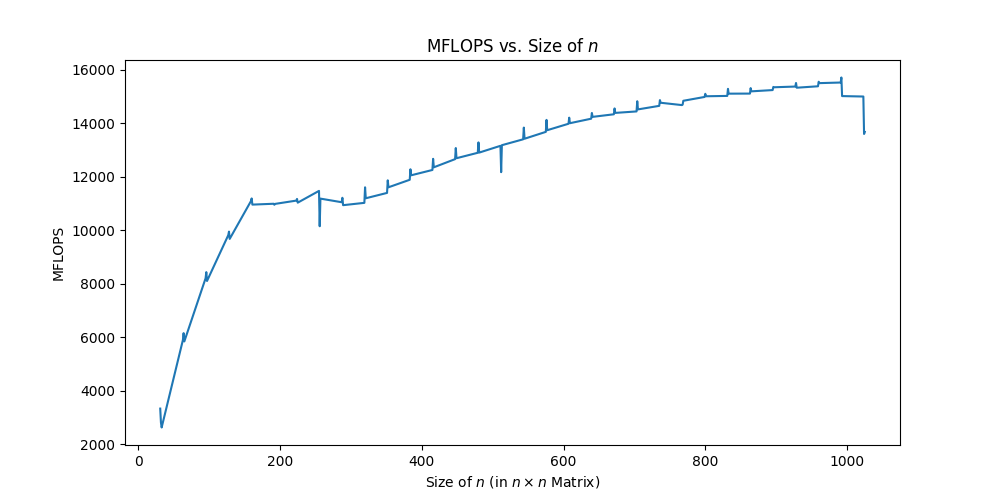
\includegraphics[width=4in]{figures/MFLOPS.png}}
  \caption{Performance Graph of Our Implementation of DGEMM}
\end{figure}

\begin{figure}
  \centerline{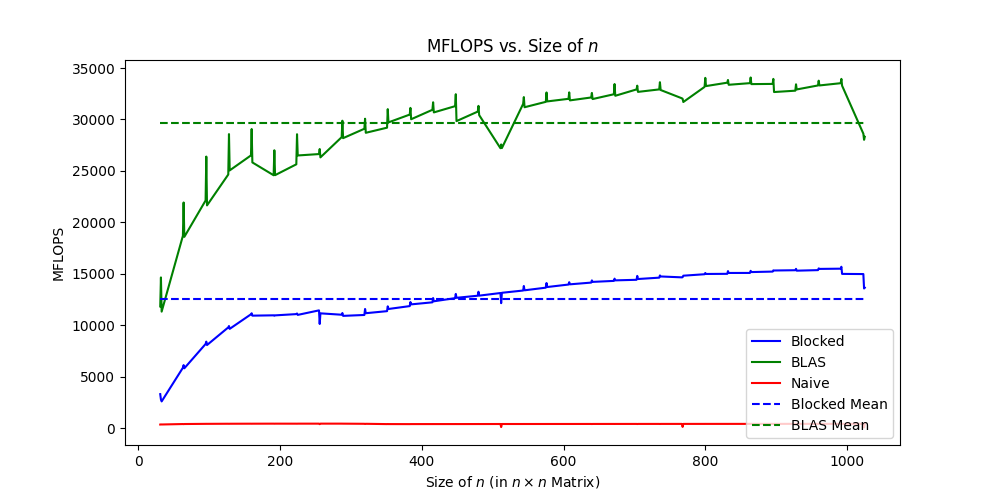
\includegraphics[width=4in]{figures/MFLOPS_compare.png}}
  \caption{Comparison of our DGEMM compared to Naive and BLAS}
\end{figure}

\begin{figure}
  \centerline{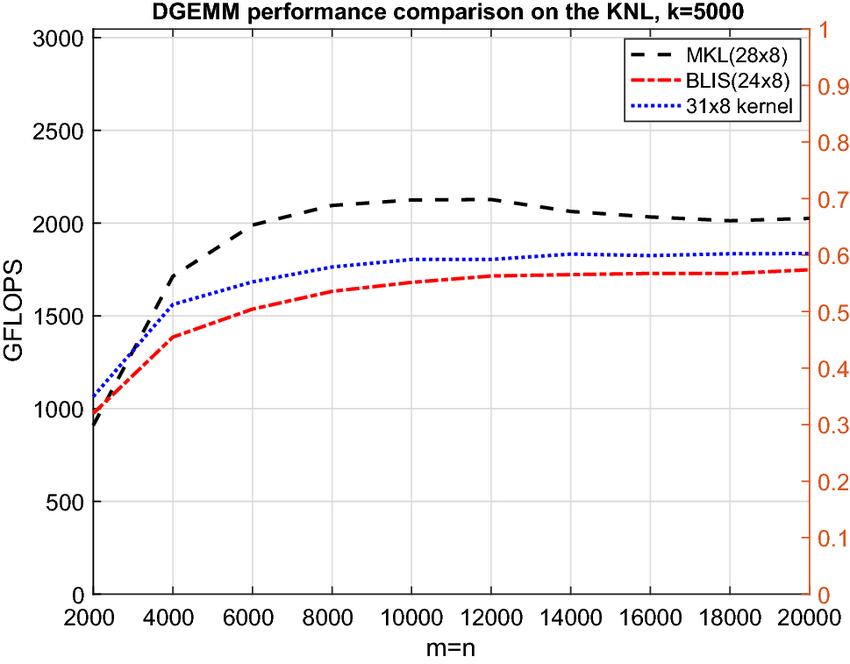
\includegraphics[width=4in]{figures/DGEMM-performance-comparison-for-different-BLAS-libraries-on-the-KNL.png}}
  \caption{Lim's Performance Graph~\cite{10.1007/s10586-018-2810-y}}
\end{figure}



\subsection{Conclusions}
The algorithm Lim uses assumes that $A, B ,C$ are all in row-major order. This was a challenge for us since we are working with column-major order matrices. Obviously, we were able to successfully work around this. We also thought about transposing the whole matrix as a whole, but were worried about the overhead cost to do that. Of course, our performance is no where near Lim's. When doing analysis and debugging of our algorithm for performance, we turned off correctness checks and just let the code run without any packing. We were able to peak around 50\% of the theoretical peak. This led us to believe that the micro kernel is indeed fast, but the design of our matrices we were given with limited how we were able to repack and transform the matrices. Given more time, we would've looked more into how to efficiently repack matrices without losing performance.

\section{General Techniques}
In this section, we'll describe our previous attempts, many of which include methods that we applied directly from reading Lim's paper~\cite{10.1007/s10586-018-2810-y}. Most of the techniques listed here helped us understand Lim's algorithm at a deeper level, allowing us to implement some version of it without needing the source code.

\subsection{Understanding the KNL Architecture}
We are using a Cori KNL node for this homework. The architecture is as follows:
\begin{lstlisting}
Architecture:        x86_64
CPU op-mode(s):      32-bit, 64-bit
Byte Order:          Little Endian
CPU(s):              272
On-line CPU(s) list: 0-271
Thread(s) per core:  4
Core(s) per socket:  68
Socket(s):           1
NUMA node(s):        1
Vendor ID:           GenuineIntel
CPU family:          6
Model:               87
Model name:          Intel(R) Xeon Phi(TM) CPU 7250 @ 1.40GHz
Stepping:            1
CPU MHz:             1401.000
CPU max MHz:         1401.0000
CPU min MHz:         1000.0000
BogoMIPS:            2800.00
L1d cache:           32K
L1i cache:           32K
L2 cache:            1024K
NUMA node0 CPU(s):   0-271
Flags:               fpu vme de pse tsc msr pae mce cx8 apic sep mtrr pge mca cmov pat pse36 clflush dts acpi mmx fxsr sse sse2 ss ht tm pbe syscall nx pdpe1gb rdtscp lm constant_tsc arch_perfmon pebs bts rep_good nopl xtopology nonstop_tsc cpuid aperfmperf pni pclmulqdq dtes64 monitor ds_cpl est tm2 ssse3 fma cx16 xtpr pdcm sse4_1 sse4_2 x2apic movbe popcnt tsc_deadline_timer aes xsave avx f16c rdrand lahf_lm abm 3dnowprefetch ring3mwait cpuid_fault epb pti intel_ppin ibrs ibpb fsgsbase tsc_adjust bmi1 avx2 smep bmi2 erms avx512f rdseed adx avx512pf avx512er avx512cd xsaveopt dtherm ida arat pln pts
\end{lstlisting}

The CPU flags indicate that we can exploit data level parallelism using at most 512 bit wide vector intrinsics. A peek into \verb|gdb| via \verb|info registers all| also shows us that a single core has a total of 32 zmm (\verb|zmm0-zmm31|) registers to be used for 512 bit wide vector operations. This knowledge of how many registers there was helpful when determining how much to unroll.. We also know that the L1 cache is 32KiB, so that means 4096 doubles can be packed inside the L1 cache. For L2 cache, that is 1024KiB or 128000 doubles. Of course, when performing optimizations, we cannot push this boundary as tightly as we can, as there are other random things in data to account for, such as data handled by the operating system for process and thread data. We can also retrieve the information of the size of a cache line:

\begin{lstlisting}
cat /sys/devices/system/cpu/cpu0/cache/index0/coherency_line_size 
64
\end{lstlisting}

This understanding of architecture also allowed us to analyze assembly code and figure out if ILP is being exploited.

\subsection{Loop Reordering}
We found that we can exploit the memory hierarchy by reordering the loops. We first focused on reordering the innermost loop, as that is the most likely to be the bottleneck. Since our matrices are in column-major order format, we found that $j, k, i$ was the most optimal ordering, giving us an average peak of 5.29\% of the peak FLOPS with a block size of 128. Because of the $j, k , i$ ordering, you can also save a memory access by storing scalar $b$ outside of the innermost for loop, as shown below. This ordering makes sense, as $A$ and $C$ can benefit from cache locality as they are both accessed in the same direction during scalar multiplication in the innermost for loop.
\begin{minted}{C}
inline static void do_block(int lda, int M, int N, int K, double* A, double* B, double* C) {
    double b;
    for (int j = 0; j < N; ++j) {
        for (int k = 0; k < K; ++k) {
            b = B[k + j * lda];
            for (int i = 0; i < M; ++i) {
                C[i + j * lda] += A[i + k * lda] * b;
            }
        }
    }
}
\end{minted}

An obvious pitfall here is that we are not exploiting (DLP) data level parallelism with SIMD, which we will explain our findings in the next section. Loop unrolling could be used to achieve ILP, but given that the x86 has 8 general and 8 floating point registers, the performance increase will be minimal or in fact decrease in our case. We think that this is due to floating point registers spilling into memory. Fortunately, unrolling will be much more feasible with AVX-512 zmm registers as there are 32 registers to utilize per iteration. Although this was one of the first and most straightforward changes, it also helped us fix minor flaws whenever we saw drops in performance, indicating we are probably missing the cache.

\subsection{Exploiting Data Level Parallelism and Utilizing AVX-512}
Next, we exploited DLP by using SIMD. The KNL node has 512 bit wide vectors, and can fit 8 double precision floating point numbers. The four intrinsics that are ideal to use are \verb|_mm512_fmadd_pd|, \verb|_mm512_set1_pd|, \verb|_mm512_load_pd|, \verb|_mm512_store_pd|. Of course, stores and loads are necessary for loading data from memory onto a SIMD register. \verb|_mm512_set1_pd| is a broadcast intrinsic, which broadcasts 1 double to a SIMD vector. \verb|_mm512_fmadd_pd| is an intrinsic that does a fused multiply add. It can do $c = c + a * b$ on each element of the SIMD vector in parallel. This is very powerful and key to a lot of other DGEMM papers using SIMD to exploit DLP, in fact the one we used in our final submission.

\begin{minted}{C}
inline static void do_block(int lda, int M, int N, int K, double* A, double* B, double* C) {
    double *buffer = _mm_malloc(8 * BLOCK, 64);
    __m512d b, c0, c1, c2, c3;

    for (int j = 0; j < N; ++j) {
        for (int i = 0; i < M && i < M / BLOCK * BLOCK; i += BLOCK) {
            memcpy(buffer, C + i + j * lda, BLOCK * sizeof(double));
            c0 = _mm512_load_pd(buffer);
            c1 = _mm512_load_pd(buffer + 8);
            c2 = _mm512_load_pd(buffer + 16);
            c3 = _mm512_load_pd(buffer + 24);
            for (int k = 0; k < K; ++k) {
                b = _mm512_set1_pd(B[k + j * lda]);
                c0 = _mm512_fmadd_pd(_mm512_load_pd(A + i + k * lda), b, c0);
                c1 = _mm512_fmadd_pd(_mm512_load_pd(A + 8 + i + k * lda), b, c1);
                c2 = _mm512_fmadd_pd(_mm512_load_pd(A + 16 + i + k * lda), b, c2);
                c3 = _mm512_fmadd_pd(_mm512_load_pd(A + 24 + i + k * lda), b, c3);
            }
            _mm512_store_pd(buffer, c0);
            _mm512_store_pd(buffer + 8, c1);
            _mm512_store_pd(buffer + 16, c2);
            _mm512_store_pd(buffer + 24, c3);
            memcpy(C + i + j * lda, buffer, BLOCK * sizeof(double));
        }
    }
    _mm_free(buffer);
}
\end{minted}

Note that in this solution, we are utilizing aligned SIMD instructions with \verb|_mm512_load_pd| and \verb|_mm512_store_pd| as opposed to \verb|_mm512_loadu_pd| and \verb|_mm512_storeu_pd|. This is because at the architectural level, moving unaligned memory to a SIMD vector could stall the instruction pipeline, since part of the memory needed could live on another cache line, thus taking extra cycles to fetch memory. 

It is also important to note that you can also take advantage of ILP. Unfortunately, unrolling more than 4 in the code above case degraded performance. We think this is related to memory, as the compiler actually does take advantage of ILP by default, by moving around intrinsics like \verb|_mm512_load_pd| and \verb|_mm512_fmadd_pd| in out of order execution. We also found that loads and stores are often costly. We believe the degradation of performance when adding more unrolling is a combination of both latency and memory stalling the CPU multiple times between each iteration. Below is a chart of latency and throughput for each intrinsic we were interested in using for this homework.

\begin{table}[ht]
\caption{Latency and Throughput of Intel Intrinsics} % title of Table
\centering % used for centering table
\begin{tabular}{c c c c} % centered columns (4 columns)
\hline\hline %inserts double horizontal lines
Intrinsic & Latency (Cycles) & Throughput (CPI) & Architecture \\ [0.5ex] % inserts table
%heading
\hline % inserts single horizontal line
\verb|_mm512_loadu_pd| & 8 & 0.5 & Skylake \\
\verb|_mm512_load_pd| & 8 & 0.5 & Skylake \\
\verb|_mm512_storeu_pd| & 5 & 1  & Skylake \\
\verb|_mm512_store_pd| & 5 & 1  & Skylake \\
\verb|_mm512_fmadd_pd| & 6 & 0.5 & KNL \\
\verb|_mm512_set1_pd| & unknown & unknown & unknown \\
[1ex] % [1ex] adds vertical space
\hline %inserts single line
\end{tabular}
\label{table:nonlin} % is used to refer this table in the text
\end{table}

Some intrinsics don't list every data on the Intel Intrinsic Guide website, so we guessed the latency and throughput from other architectures, such as Skylake. Loads seem to be the most costly, yet provide a high throughput (lower CPI is better). Same goes for fused multiply add intrinsic. We figured that in order to improve latency costs, it's better to unroll as much as possible to overcome these overheads. We also know that KNL is a superscalar architecture, meaning that in our case, two SIMD instructions can operate at the same time.

\section{Contributions}
Brian was able to start off the homework with a few implementations that peaked at 11.1\%. Realizing how different the architecture was, we had to search other optimizations that were more specific to KNL architecture. Luckily, Brian was able to come across and share Lim's paper and its description of optimizations used specifically for the KNL architecture. Michael was able to code most of the implementation from Lim's paper. Most of the contribution to the current implementation that achieves 28.14\% peak performance goes to Michael. Brian was helpful with debugging and pinpointing any fallacies within the code in terms of performance. Iniyaal was unresponsive to the group chat and didn't share any code. She has not contributed or committed to our group repository at all.

\bibliographystyle{ieeetr}
\bibliography{references} 
\end{document}
